\documentclass{standalone}
\usepackage{tikz,amsmath}
\begin{document}
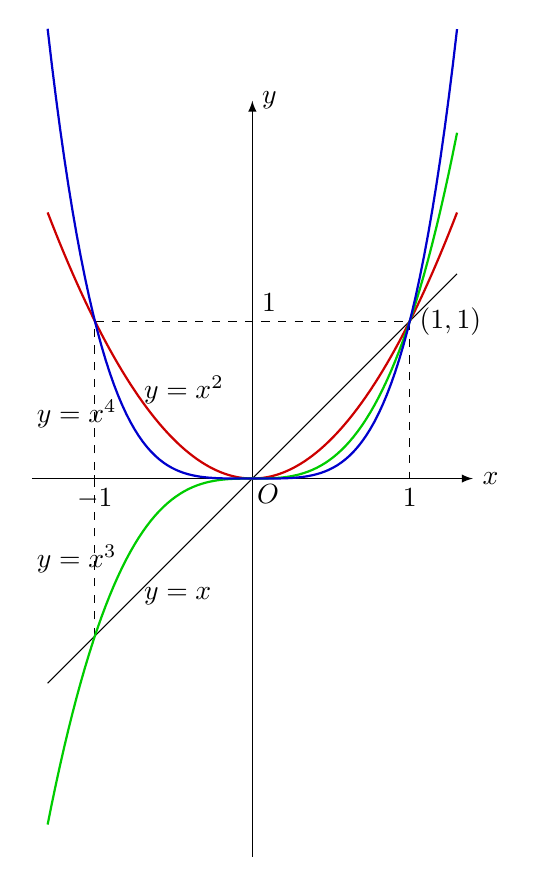
\begin{tikzpicture}[>=latex, scale=2]
  \draw[->] (-1.4,0)--(1.4,0)node[right]{$x$};
  \draw[->] (0,-2.4)--(0,2.4)node[right]{$y$};
\foreach \x in {-1,1}
{
\draw (\x,0)node[below]{$\x$}--(\x,.02);
}
\node at (.1,-.1){$O$};
\draw[dashed](-1,-1)--(-1,1)--(1,1)--(1,0);

\draw (-1.3,-1.3)--(1.3,1.3);
\draw [domain=-1.3:1.3, samples=100, thick,red!80!black]plot(\x, {\x*\x});
\draw [domain=-1.3:1.3, samples=100, thick,green!80!black]plot(\x, {\x*\x*\x});
\draw [domain=-1.3:1.3, samples=100, thick,blue!80!black]plot(\x, {\x*\x*\x*\x});
\node at (0,1)[above right]{1};
\node at (1,1)[right]{$(1,1)$};
\node at (-.75,-.75)[right]{$y=x$};
\node at (-.8,-.512)[left]{$y=x^3$};
\node at (-.75,.5625)[right]{$y=x^2$};
\node at (-.8,.41)[left]{$y=x^4$};
      \end{tikzpicture}
\end{document}